% This is samplepaper.tex, a sample chapter demonstrating the
% LLNCS macro package for Springer Computer Science proceedings;
% Version 2.20 of 2017/10/04
%
\documentclass[runningheads]{llncs}
%
\usepackage{graphicx}
\usepackage{xspace}
\usepackage{comment}
\usepackage{standalone}
\usepackage{xcolor}
\usepackage{multirow}
\usepackage{mathtools}
\usepackage[inline]{enumitem}
\usepackage{amsmath}
\usepackage{amssymb}
\usepackage{xifthen}
\usepackage[chorus]{emf}
%\usepackage{mathabx}
%\usepackage{unicode-math}
%SAVING SPACE
\usepackage[moderate]{savetrees}

\begin{comment}
Potential Conferences:
Research
=========
- http://www.guide2research.com/conference/wims-2020
-https://cikm2020.org/call-for-papers-full-and-short-research-papers/
- http://wi2020.vcrab.com.au/
- ISWC: Deadline: 27 March, Content: Formalization + Approach global
- Web Intelligence: 1 June
- CIKM: http://www.cikmconference.org/, Deadline: 1 May

Demo
=====
- ESWC, Deadline: March 12, 2020
- ISWC 

Journal
=======

Work Plan
==========
Week1: Formalization
Week2: Experimentation


February: Complex 
\end{comment}



%below figure
%\setlength{\belowcaptionskip}{-15pt}

% Used for displaying a sample figure. If possible, figure files should
% be included in EPS format.
%
% If you use the hyperref package, please uncomment the following line
% to display URLs in blue roman font according to Springer's eBook style:
\PassOptionsToPackage{hyphens}{url}
\usepackage[hidelinks]{hyperref}
\renewcommand\UrlFont{\color{blue}\rmfamily}
\newcommand\bigforall{\mbox{\Large $\mathsurround0pt\forall$}}
 \newcommand\bigexist{\mbox{\Large $\mathsurround0pt\exists$}} 
 \newcommand\bigCurlyO{\mbox{\Large $\mathsurround0pt \{$}} 
 \newcommand\bigCurlyC{\mbox{\Large $\mathsurround0pt \}$}} 
  
  \newcommand\bigParO{\mbox{\Large $\mathsurround0pt($}}
  \newcommand\bigParC{\mbox{\Large $\mathsurround0pt)$}}
  
\definecolor{nbColor}{rgb}{0,0,1}
\definecolor{nhColor}{rgb}{0,0.5,0.2}
\definecolor{anycolor}{rgb}{1,0.5,0.2}
\newcommand{\nb}[1]{\textcolor{nbColor}{\textbf{[nb: #1]}}}
\newcommand{\nath}[1]{\textcolor{nhColor}{\textbf{[nh: #1]}}}
\newcommand{\coment}[2]{\textcolor{anycolor}{\textbf{[#1: #2]}}}



\newcommand{\pow}[1]{\ensuremath{2^{#1}}\xspace}
\newcommand{\IRI}{\ensuremath{\mathbf{IRI}}\xspace}
\newcommand{\Lit}{\ensuremath{\mathbf{L}}\xspace}
\newcommand{\thingin}{\textit{Thing~in}\xspace}
\newcommand{\lstref}[1]{Listing~\ref{lst:#1}}
\newcommand{\lstRefline}[2]{Listing~\ref{lst:#1}, Line~\ref{line:#2}}
\newcommand{\appref}[1]{Appendix~\ref{app:#1}}
\newcommand{\reftab}[1]{Table~\ref{tab:#1}}
\newcommand{\tabref}[1]{Table~\ref{tab:#1}}
\newcommand{\secref}[1]{Section~\ref{sec:#1}}
\newcommand{\qref}[1]{~\ref{eq:#1}}
\newcommand{\figref}[1]{Figure~\ref{fig:#1}}
\newcommand{\figRefPart}[2]{Figure~\ref{fig:#1} (#2)}
\newcommand{\kword}[1]{\ensuremath{\texttt{#1}}}
\newcommand{\prefixWord}[1]{\texttt{#1}}
\newcommand{\cf}{\textit{cf.} \xspace}
\newcommand{\dataelement}{\textit{data element}\xspace}
\newcommand{\dataelements}{\textit{data elements}\xspace}
\newcommand{\rawData}{\figref{sampleRawData}\xspace}
\newcommand{\refParkingData}{\figref{sampleRawData}\xspace}

\newcommand{\wrt}{with respect to\xspace}



\newcommand{\schemaType}{\textit{schema type}\xspace}
\newcommand{\schemaElements}{\textit{schema elements}\xspace}
\newcommand{\schemaElement}{\textit{schema element}\xspace}

\newcommand{\simpleSchema}{\textit{simple schema}\xspace}
\newcommand{\simpleSchemas}{\textit{simple schema}s\xspace}
\newcommand{\SimpleSchema}{\textit{Simple schema}\xspace}
\newcommand{\SimpleSchemas}{\textit{Simple schemas}\xspace}


%minimally connected simple ontology structure
\newcommand{\connectedOntologyStructure}{\textit{type property path structure}\xspace}
\newcommand{\ConnectedOntologyStructure}{\textit{Type property path structure}\xspace}


\newcommand{\descriptionVocabulary}{\textit{Description vocabulary}\xspace}

\newcommand{\elementVocabulary}{\textit{Element vocabulary}\xspace}
\newcommand{\finalMapping}{\textit{Final mapping}\xspace}

\newcommand{\frontendMA}{\textit{Front-end mapping application}\xspace}
\newcommand{\vocabPathGen}{\textit{Vocabulary path generator}\xspace}
\newcommand{\DataPropertyPath}{\textit{Data property path}\xspace}
%Simple ontology structure
%==========================
\newcommand{\vocabularyStructure}{\textit{Vocabulary structure}\xspace}

%Schema Description
%==================
\newcommand{\schemaDescription}{\textit{schema description}\xspace}
\newcommand{\schemaDescriptions}{\textit{schema descriptions}\xspace}

%Mapping Generation System
%==========================
\newcommand{\mappingGenerationSystem}{\textit{mapping generation system}\xspace}
\newcommand{\MappingGenerationSystem}{\textit{Mapping generation system}\xspace}


\newcommand{\defref}[1]{Definition~\ref{def:#1}}

\newcommand{\Eo}{\ensuremath{\emf}\xspace}
\newcommand{\Co}{\ensuremath{\mathcal{C}}\xspace}
\newcommand{\Po}{\ensuremath{\mathcal{P}}\xspace}
\newcommand{\Do}{\ensuremath{\mathcal{D}}\xspace}
\newcommand{\del}{\ensuremath{\mathcal{\delta}}\xspace}
\newcommand{\So}{\ensuremath{\mathcal{S}}\xspace}

\newcommand{\minScore}{\ensuremath{minScore}\xspace}
\newcommand{\maxEntity}{\ensuremath{maxEntity}\xspace}

\newcommand{\subOnt}{\ensuremath{\subseteq}\xspace}

\newcommand{\R}{\ensuremath{\mathbb{R}}\xspace}
\newcommand{\Z}{\ensuremath{\mathbb{Z^{+}}}\xspace}


\newcommand{\resref}[1]{Result~\ref{res:#1}}

\newcommand{\tuple}[1]{\ensuremath{\langle#1\rangle}}

\newcommand{\bOc}{\ensuremath{\big{\{}}}
\newcommand{\bCc}{\ensuremath{\big{\}}}}

%Symbols in formalization
\newcommand{\symSimpleSchema}[1]{\ensuremath{\ifthenelse{\isempty{#1}}{\sigma}{\sigma_#1}}\xspace}

\newcommand{\symTypeDescription}[1]{\ensuremath{\ifthenelse{\isempty{#1}}
		{\mathfrak{t}\xspace}{\mathfrak{t}_#1}\xspace}}
	
\newcommand{\symElementsDescription}[1]{\ensuremath{\ifthenelse{\isempty{#1}}
		{\mathcal{E}\xspace}{\mathcal{E}_#1}\xspace}}
	
\newcommand{\symOntology}[1]{\ensuremath{\ifthenelse{\isempty{#1}}
		{v\xspace}{v_#1}\xspace}}

\newcommand{\symSchemaSet}{\ensuremath{\mathbb{S}\xspace}}
\newcommand{\symOntologySet}{\ensuremath{\mathbb{V}\xspace}}
\newcommand{\symOntologyMerge}{\ensuremath{\uplus}\xspace}
\newcommand{\symSchemaDescriptionSet}{\ensuremath{\mathbb{D}}\xspace}
\newcommand{\symSubVocabulary}{\ensuremath{\;\underline{\Subset}\;}\xspace}

\newcommand{\symSimCal}{\ensuremath{f_s}\xspace}
\newcommand{\symConMap}{\ensuremath{f_c}\xspace}
\newcommand{\symPathDesGen}{\ensuremath{f_e}\xspace}
\newcommand{\symSchemaDes}{\ensuremath{f_d}\xspace}
\newcommand{\symProb}{\ensuremath{\R}\xspace}

\newcommand{\symPathGen}{\ensuremath{f_v}\xspace}
\newcommand{\symPath}{\ensuremath{\mathfrak{p}}\xspace}
\newcommand{\symTriple}{\ensuremath{\mathfrak{t}}\xspace}

\newcommand{\symMappedElements}{\ensuremath{\Sigma}\xspace}
\newcommand{\symElementOntologies}{\ensuremath{\Theta}\xspace}

\newcommand{\Dso}{\ensuremath{\delta}\xspace}
\newcommand{\Rso}{\ensuremath{r}\xspace}




\makeatletter
\providecommand*{\cupdot}{%
	\mathbin{%
		\mathpalette\@cupdot{}%
	}%
}
\newcommand*{\@cupdot}[2]{%
	\ooalign{%
		$\m@th#1\bigcup$\cr
		\hidewidth$\m@th#1\bullet$\hidewidth
	}%
}
\makeatother
\usepackage{xcolor}
\definecolor{babyblueeyes}{rgb}{0.63, 0.79, 0.95}
\usepackage{colortbl}

\newcolumntype{g}{>{\columncolor[gray]{0.8}}c}
\newcolumntype{t}{>{\columncolor{babyblueeyes}}c}

\begin{document}
%
%\title{Semi-automatic RDFization of data in heterogeneous formats\thanks{Supported by organization x.}}
\title{Semi-automatic RDFization using automatically generated mappings}

%


%\titlerunning{Abbreviated paper title}
% If the paper title is too long for the running head, you can set
% an abbreviated paper title here
%
\author{Noorani Bakerally\inst{1,2}\underline{\underline{}}\and
Cyrille Bareau\inst{3} \and Fabrice Blache\inst{3} \and Sébastien Bolle\inst{3} \and Christelle Ecrepont\inst{2} \and Pauline Folz\inst{3} \and Nathalie Hernandez\inst{1} \and Thierry Monteil\inst{2}  \and Gilles Privat\inst{3} \and Fano Ramparany\inst{3}}

%
\authorrunning{N. Bakerally et al.}
% First names are abbreviated in the running head.
% If there are more than two authors, 'et al.' is used.
%
\institute{IRIT, Toulouse, France \email{\{firstname.lastname\}@irit.fr} \and
LAAS-CNRS, National Institut of applied Sciences of Toulouse, Toulouse 31400,
\email{\{firstname.lastname\}@laas.fr}\\
\url{http://www.springer.com/gp/computer-science/lncs} \and
Orange Labs, Meylan, France\\
\email{\{firstname.lastname\}@orange.com}}
%
\maketitle              % typeset the header of the contribution
%
\begin{abstract}
Most data available on the Web do not conform to the RDF data model. A number of tools/approaches have been developed to encourage the transition to RDF. Manual and automatic tools/approaches tend to be complex and rigid respectively. On the other hand, semi-automatic tools can hide and automate complex tasks while enhancing flexibility by solicitating human experts for decision making purposes. In this paper, we describe a semi-automatic approach to facilitate the transformation of heterogeneous semi-structured data to RDF. We provide an implementation of our approach and demonstrate its use using real datasets from ppen data portals.


%The originality of our contribution is that it automatically generates several holistic mappings and try best to provide an exhaustive description for a given type of instances. We provide the foundation and motivation for such a contribution and describe the approach. Finally, we describe an implementation of the approach and validate it by performing several experiments on real datasets from city open data portals.


%They mainly include mapping languages and semi-automatic tools.
%Mapping languages tend to have a steep learning curve as they require knowing the syntax and semantics of the languages in addition to the Semantic Web stack and ontologies that can be used. 
\keywords{RDF, Data transformation, Semi-automatic approach}
\end{abstract}
%
%
%
\input{whole.tex}
\section{Introduction}

To realize the vision of the Semantic Web, the conformance of existing data to the RDF model is a necessary condition. Yet, it is a fact that most of the data available on the Web do not satisfy the latter requirement. A number of tools have been developed to facilitate the transition to RDF. Much of them are founded on well-defined mapping languages (R2RML~\cite{R2RML_W3C:12}, RML~\cite{dimou2014rml}, SPARQL-Generate~\cite{lefranccois2016flexible}, etc.). Using mapping languages directly is complex. This is because they have a steep learning curve and require knowing the syntax and semantics of the languages in addition to the Semantic Web stack and ontologies that can be used. 

Besides mapping languages, there are automatic and semi-automatic RDFizers. We ignore automatic RDFizers (e.g. Direct Mapping~\cite{Direct_Mapping_W3C:12}, Docker2RDF~\cite{ayed2017docker2rdf}, etc.) as their transformation cannot be customized or they are restricted for specific domain models. The minor category of works (RMLEditor~\cite{heyvaert2016rmleditor}, OpenRefine~\cite{verborgh2013using}) around semi-automatic RDFizers is our main interest. We focus on this category due to their ability in aiding human experts by automating complex tasks without hindering flexibility by incorporating them for decision making and validation. The main problem with the latter tools is that they mostly only provide a graphical interface with some facilities for searching through ontologies. However, they depend much on human experts with respect to knowledge about ontologies and data modeling using them.

In this work, our aim is to provide an approach to further facilitate semi-automatic RDFizers by automatically generating initial mappings that may then be customized by human experts. The originality of our contribution is that it automatically generates several holistic mappings and try best to provide an exhaustive description for a given type of instances. Our approach is not an alternative but complementary to existing tools. In the rest of this paper, we describe our approach and its implementation in \secref{approach} and \secref{implementation} respectively. Finally, we demonstrate our implementation using real datasets from open data portal. %Finally, we describe \secref{futureWork} that are we are currently working on.   



\section{Our Approach}\label{sec:approach}
Our approach to generate initial mappings consists of four main steps as shown in \figref{overviewApproach}. For illustration purposes, we consider a parking dataset\footnote{\url{http://data.metropolegrenoble.fr/ckan/dataset/parkings-de-grenoble/resource/a6919f90-4c38-4ee0-a4ec-403db77f5a4b}, last accessed on 7 December 2019} from Grenoble open data portal\footnote{\url{http://data.metropolegrenoble.fr/}, last accessed on 7 December 2019}. \figref{sampleRawData} is part of a preview of that dataset taken directly from the data portal.

\begin{figure}[h]
	\centering
	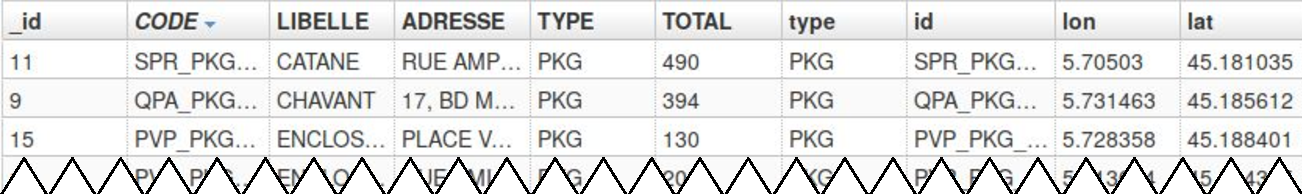
\includegraphics[scale=0.45]{images/sampleRawData.pdf}
	\caption{Parking data from Grenoble Open Data Portal}
	\label{fig:sampleRawData}
\end{figure}

Moreover, our approach uses an \kword{Ontology repository}. Suppose that it contains the vocabularies MobiVoc\footnote{\url{https://www.mobivoc.org/}, last accessed 10 February 2020}, Schema.org\footnote{\url{https://schema.org/}, last accessed 10 February 2020}, WGS84\footnote{\url{https://www.w3.org/2003/01/geo/}, last accessed 10 February 2020} and Dublin Core Metadata Terms\footnote{\url{https://www.dublincore.org/specifications/dublin-core/dcmi-terms/}, last accessed 10 February 2020}. 

\begin{figure}
	\centering
	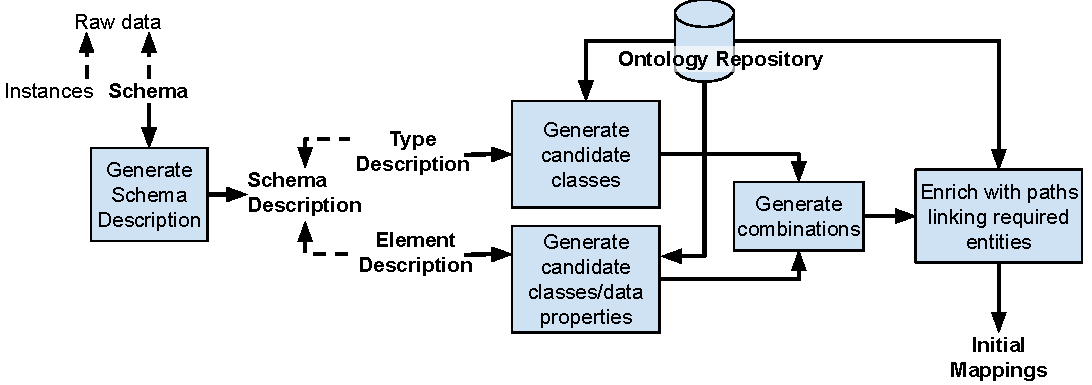
\includegraphics[scale=0.55]{images/GeneralApproachPaper1.pdf}
	\caption{Mappings Generation Process}
	\label{fig:overviewApproach}
\end{figure}

In our approach, to capture the background knowledge about the schema used in the raw data, firstly, we generate a \kword{Schema description} consisting of a \kword{Type description} and a \kword{Elements description}. \kword{Type Description} characterizes using keywords the type of objects described by the schema. \kword{Elements description} characterizes using keywords the schema elements (e.g. \kword{lon} in \figref{sampleRawData}).   


Secondly, using an \kword{Ontology repository}, and the \kword{Type description} and the \kword{Elements description}, a set of candidate classes are generated for typing objects and a set of candidate data properties or classes are generated for modeling the schema element. 

\tabref{overviewElementMappings} shows a schema description for the schema of \figref{sampleRawData} and generated ontology entities for its elements. For example, the objects' type in \figref{sampleRawData} can be described by the keyword `parking facility'. Using the latter description, the classes \kword{mv:ParkingFacility} and \kword{sc:Park} are generated to type the objects. Similarly, the schema element \kword{TOTAL} is described using the keywords `capacity' and `total' using which the class \kword{mv:Capacity} and data property \kword{sc:totalTime} are candidate classes generated to model it. The candidate proposal \kword{sc:totalTime} is not appropriate to model \kword{TOTAL} as its semantics is not compatible with the latter. To determine the appropriateness of an entity, we also generated a confidence. For simplicity sake, we omit this information from \tabref{overviewElementMappings}.




\begin{comment}
For example, suppose the \kword{Type Description} include the keyword `parking facility' to describe the objects' type in \figref{sampleRawData}. This description is used to generate candidate classes that include \kword{mv:ParkingFacility} and \kword{sc:Park}.

Similarly, suppose the \kword{Elements Description} for the schema element \kword{TOTAL} and \kword{lon} in \figref{sampleRawData} include the keywords `capacity' and `longitude' respectively.

Using these descriptions, the candidate classes and data property generated for \kword{TOTAL} include \kword{mv:Capacity} and \kword{sc:totalTime} respectively.

Similarly, the candidate data property generated for \kword{lon} is \kword{wgs84:long}.
\end{comment}


%\vspace{-0.5cm}
\begin{table}[]
	\centering
	\scalebox{0.7}{
		\begin{tabular}{|l|l|l|l|l|}
			\hline
			\multicolumn{3}{|c|}{\textbf{Schema Description}}                                                                         & \multicolumn{2}{c|}{\textbf{Generated Entities}}                                                 \\ \hline
			&          & \textbf{Keyword}   & \textbf{Classes}                                                      & \textbf{Data Properties} \\ \hline
			\textbf{\begin{tabular}[c]{@{}l@{}}Type \\ Description\end{tabular}}                      &          & `parking facility' & \begin{tabular}[c]{@{}l@{}}\kword{mv:ParkingFacility},\\ \kword{sc:Park}\end{tabular} &                          \\ \hline
			\multirow{6}{*}{\textbf{\begin{tabular}[c]{@{}l@{}}Elements \\ Description\end{tabular}}} & \kword{id}       & `identifier'       &                                                                       & \kword{dc:identifier}            \\ \cline{2-5} 
			& \kword{LIBELLE}  & `description'      &                                                                       & \kword{sc:description}           \\ \cline{2-5} 
			& \kword{TOTAL}    & `capacity',`total' & \kword{mv:Capacity}                                                           & \kword{sc:totalTime}             \\ \cline{2-5} 
			& \kword{lat}      & `latitude'         &                                                                       & \kword{wgs84:lat}                \\ \cline{2-5} 
			& \kword{lon}      & `longitude'        &                                                                       & \kword{wgs84:long}               \\ \cline{2-5} 
			& \kword{ADDRESSE} & `address'          &                                                                       & \kword{sc:address}               \\ \hline
	\end{tabular}}
	\caption{Candidate entities for typing and schema elements}
	\label{tab:overviewElementMappings}
\end{table}
%\vspace{-1cm}


Thirdly, possible combinations are generated. A combination consists of a candidate class for typing, that we refer as the \emph{type class}, and a candidate data property or class for each schema element if it was generated in the previous step. \tabref{overviewCombinationsElements} shows all combinations generated from the candidate entities in \tabref{overviewElementMappings}. As we can see, in each combination, there is one candidate entity for the type class and schema elements.

%\vspace{-0.5cm}
\begin{table}[]
	\centering
	\scalebox{0.7}{
		\begin{tabular}{|l|l|l|l|l|l|l|l|}
			\hline
			& \textbf{Type Class} & \textbf{id}   & \textbf{LIBELLE} & \textbf{TOTAL} & \textbf{lat} & \textbf{lon} & \textbf{ADDRESSE} \\ \hline
			1. & \kword{mv:ParkingFacility}  & \kword{dc:identifier} & \kword{sc:description}   & \kword{mv:Capacity}    & \kword{wgs84:lat}    & \kword{wgs84:lon}    & \kword{sc:address}        \\ \hline
			2. & \kword{mv:ParkingFacility}  & \kword{dc:identifier} & \kword{sc:description}   & \kword{sc:totalTime}   & \kword{wgs84:lat}    & \kword{wgs84:lon}    & \kword{sc:address}        \\ \hline
			3. & \kword{sc:Park}             & \kword{dc:identifier} & \kword{sc:description}   & \kword{mv:Capacity}    & \kword{wgs84:lat}    & \kword{wgs84:lon}    & \kword{sc:address}        \\ \hline
			4. & \kword{sc:Park}             & \kword{dc:identifier} & \kword{sc:description}   & \kword{sc:totalTime}   & \kword{wgs84:lat}    & \kword{wgs84:lon}    & \kword{sc:address}        \\ \hline
	\end{tabular}}
	\caption{Combinations of generated entities for type class and schema elements}
	\label{tab:overviewCombinationsElements}
\end{table}
%\vspace{-1cm}

Finally, we enrich each combination with the required ontology entities to instantiate them for every object in the raw data. For example, \figref{combinationNoPath} shows the first combination from \tabref{overviewCombinationsElements} and the required paths, illustrated as dotted lines, that will be generated at this step. It is possible that there may be more than one paths or no paths between some entities. A combination and the required paths makes up one initial mapping. To choose an initial mapping and further customize it by choosing and validating the paths, a user interface is provided.

%\figref{sampleOntologyRawData} is a possible result with some of the paths generated. 



%For example, in the third combination from \tabref{overviewCombinationsElements}, there may be no path between the type class \kword{sc:Park} and the candidate class of \kword{TOTAL} that is \kword{mv:Capacity} . In this case, a human expert may chose to ignore this mapping     

%\vspace{-0.5cm}
\begin{figure}
	\centering
	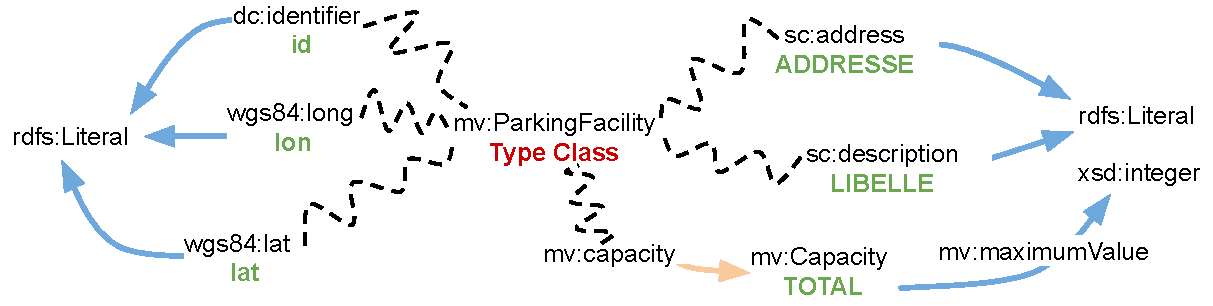
\includegraphics[scale=0.4]{images/combinationNoPath.pdf}
	\caption{Final mapping for first combination without generated paths}
	\label{fig:combinationNoPath}
\end{figure}
%\vspace{-1cm}

\section{Implementation}\label{sec:implementation}
An overview of our implementation is shown in \figref{OverviewImplementation}. Core to this implementation is the \kword{RDFizer} that generate initial mappings using the approach described in the previous section. To facilitate human intervention,
we provide a graphical \kword{User Interface}. Using the interface, users can upload the raw data in the CSV format and may enrich it with keywords to generate the \kword{Schema description}. The \kword{User Interface} interacts with the \kword{RDFizer} via a \kword{Web Service}. Eventually, on obtaining the initial mappings, one of them is chosen and, refined and validated by the human expert and sent to the web service together with the raw data for transformation to RDF.

\begin{figure}[h]
	\centering
	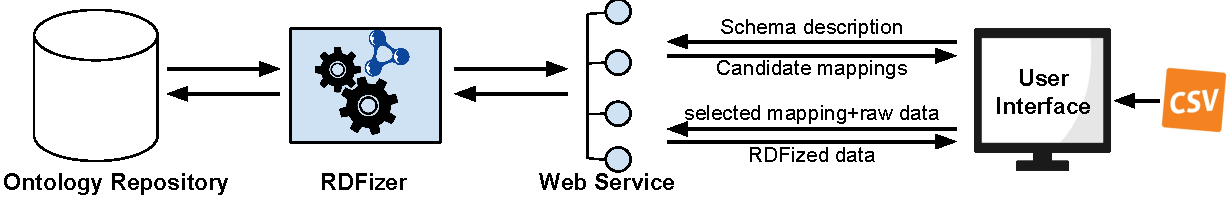
\includegraphics[scale=0.55]{images/OverviewImplementation.pdf}
	\caption{Overview of Implementation}
	\label{fig:OverviewImplementation}
\end{figure}

The user interface is a web application implemented using the JavaScript library \emph{React}\footnote{\url{https://reactjs.org/}}. The video shows the use the interface to generate mappings for the CSV parking dataset in \secref{approach}. As it can be seen, the user interface (\figref{screenshotInterface}) has three main parts. The top left part is focused on the raw data that is imported using the \kword{import CSV} menu item. On clicking on a column, keywords can be entered. The bottom left part shows the initial mappings and on selecting one of them, its corresponding description graph is rendered on the right part. The human expert can interact with different part of the latter graph and select and validate the paths. 

%For each possible mapping in the bottom right part, different pieces of information are provided namely: score, type class, number of classes/data properties and finally number of (un)mapped columns. Two main refinements are possible for each possible mapping. Firstly, data properties can be specified in class mappings. Secondly, ontology entities can be changed and paths can be re-generated for any schema element. This gives the user full flexibility to change and adapt a particular possible mapping.     


\begin{figure}[h]
	\centering
	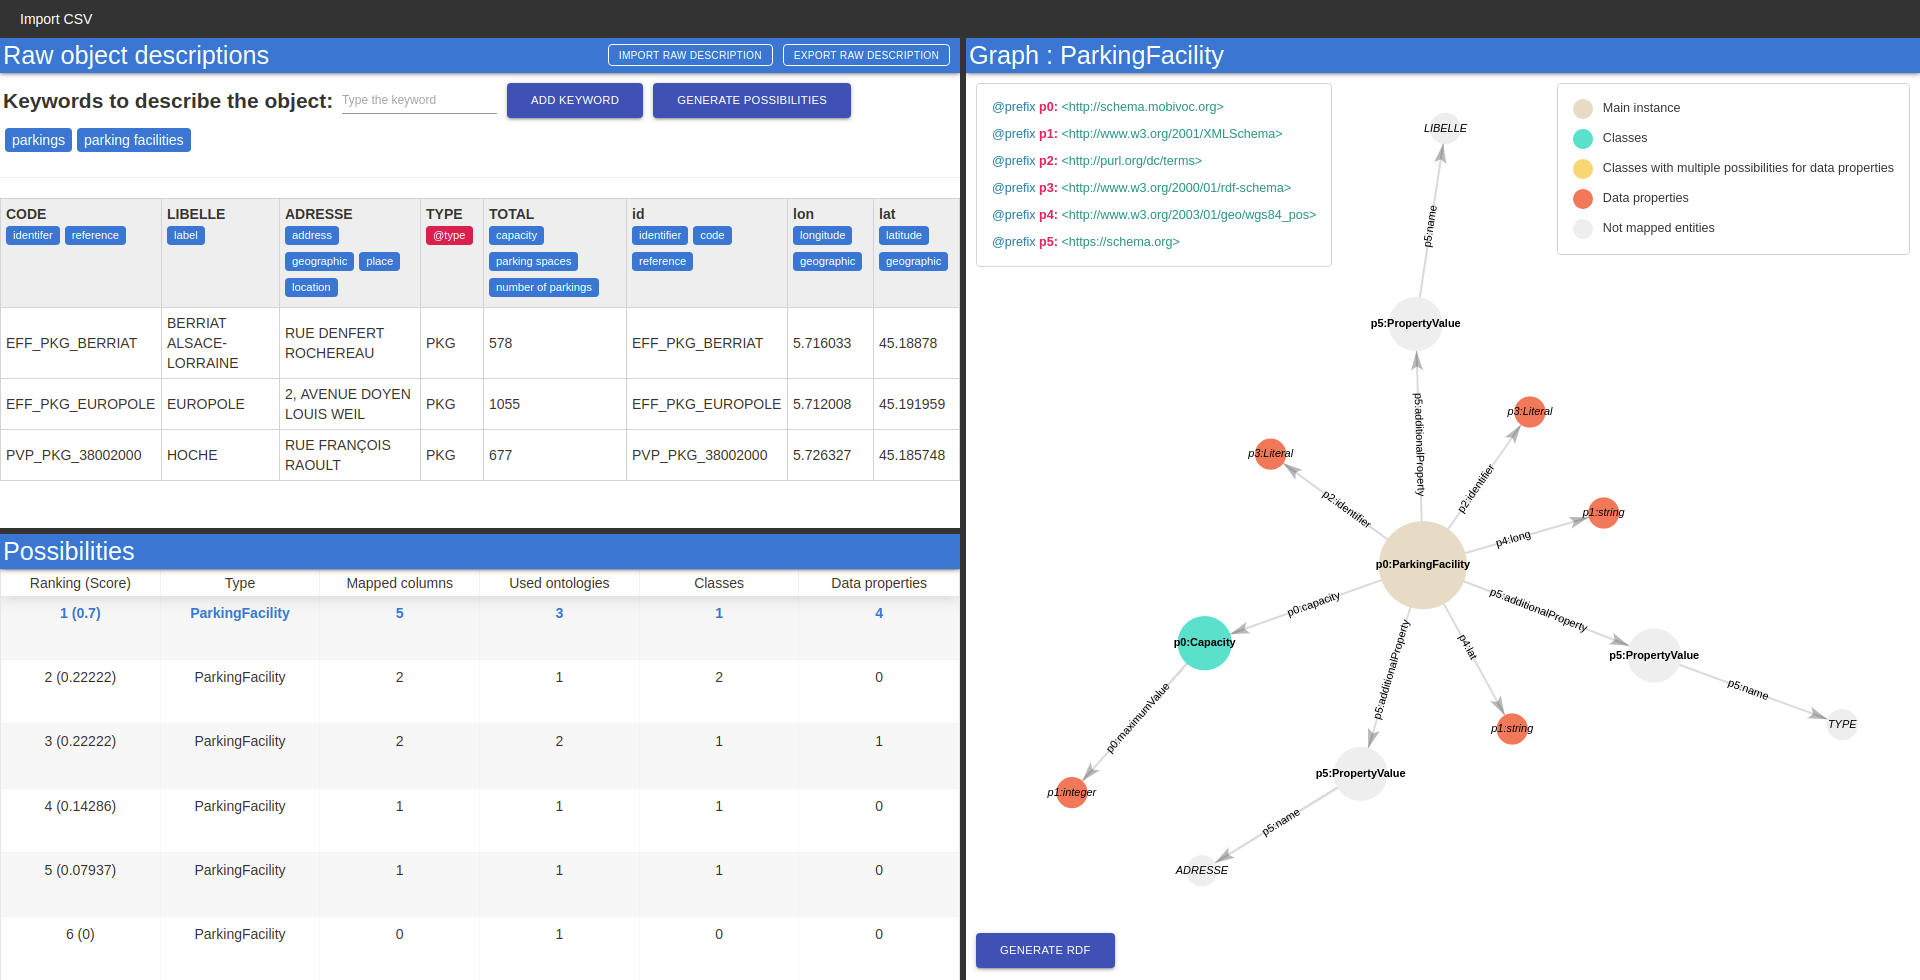
\includegraphics[scale=0.15]{images/global.png}
	\caption{Screenshot of user interface}
	\label{fig:screenshotInterface}
\end{figure}

\section{Demonstration}\label{sec:demonstration}
Our demonstration consist of using datasets from open data portals for some cities in France. \figref{expMappingParking} shows some of our experiments using these datasets. For each city, we performed two experiment. In \kword{NK}, no keywords are added by the user while in \kword{WK}, keywords are added. As we can see, even without keywords, there are fields that can be correctly mapped. Obviously, with keywords, initial mappings with better quality are generated. For all these datasets, we have their respective schema descriptions that we intend to use in our demonstration. 



\begin{figure}
	\centering
	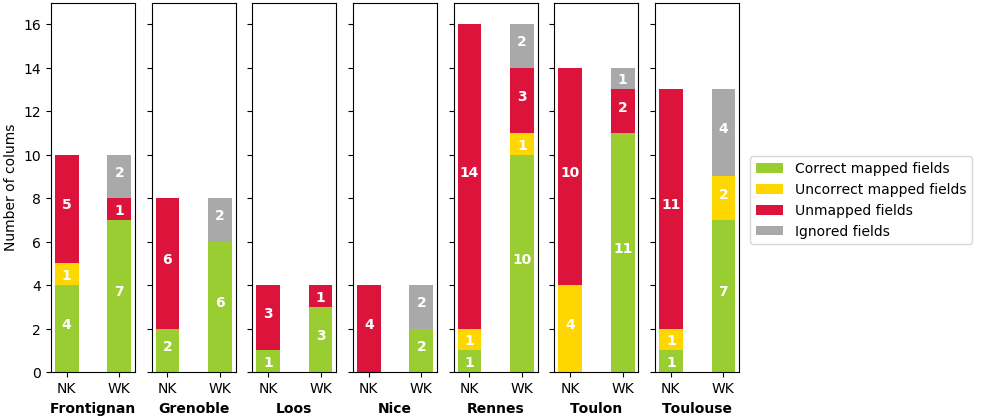
\includegraphics[scale=0.3]{./images/mappingPerParking1.png}
	\caption{Mappings of the columns grouped per parking dataset. Where \emph{NK} represents the 
		experiment without keywords and \emph{WK} represents the experiments with keywords.}
	\label{fig:expMappingParking}
\end{figure}










%\section{Motivations and Foundations}\label{sec:foundationMotivation}
In this section, we describe the motivation and foundations of our work. More specifically, we present the context of our work in \secref{context}. \secref{requirements} describes the requirements that we have used when assessing related works in the literature. In \secref{relatedWork}, we describe related works and how they are failing to satisfy our requirements. Finally, \secref{illustratingScenario} describes an illustrating scenario that we use throughout this paper.  

\subsection{Context}\label{sec:context}
This work takes place in a private collaboration between the Orange and the french laboratories LAAS and IRIT. It revolves around the \thingin\footnote{\url{https://hellofuture.orange.com/en/thingin-the-things-graph-platform/}, last accessed 7 December 2019} platform whose aim is to maintain thorough structural and semantic description of the environments, such as cities or buildings, containing objects that may be inter-related between themselves. While \thingin is based on NGSI-LD\footnote{\url{https://www.etsi.org/newsroom/press-releases/1519-2019-01-etsi-cim-group-releases-full-feature-specification-for-context-information-exchange-in-smart-cities}},on a high-level information model, it supports import and export RDF data.

\figref{contextThingIn} shows the positioning of \thingin in an Internet of Things (IoT) ecosystem. In such an ecosystem, there are objects of different kinds such as \kword{IoT devices} (e.g. sensors, actuators) and \kword{non-connected objects} (e.g. tables, chairs) . For multiple reasons, such as different protocols, standards, there is a heterogeneity of \kword{IoT platforms} for managing  devices. Consequently, there may be no single entrypoint to access description of objects. In this situation, \thingin can homogenize access to these descriptions by acting as a directory of objects.

\begin{figure}[h]
	\centering
	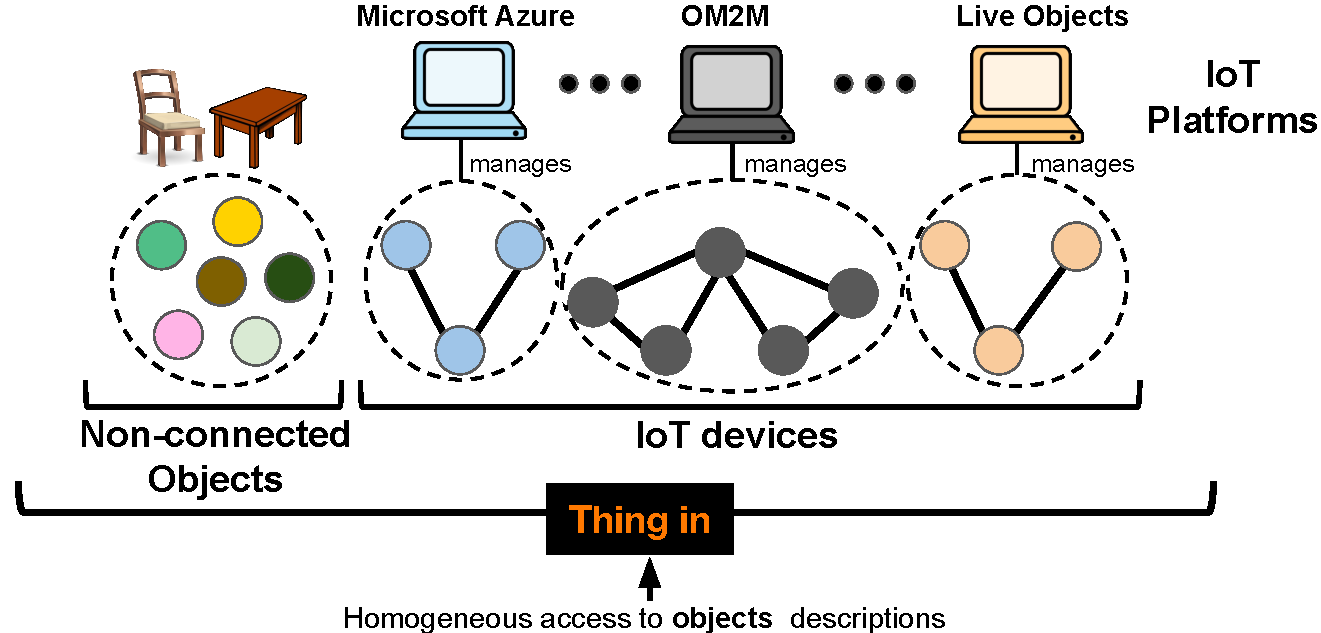
\includegraphics[scale=0.5]{images/contextThingIn.pdf}
	\caption{\thingin in an IoT ecosystem}
	\label{fig:contextThingIn}
\end{figure}

For \thingin to be used as a catalog of objects, it must contain their descriptions. However, importing these descriptions into it is problematic as they are heterogeneous due to the diversity of data formats and domain models that exist. As mentioned above, \thingin can import data in RDF. This is where the task of facilitating the transformation of heterogeneous semi-structured data to RDF comes into play.



\subsection{Requirements}\label{sec:requirements}
Before moving on to related works, let us explicitly mention the requirements used when considering these works. We require that an approach:

\paragraph{\textbf{R1. does not necessitate prior knowledge of existing ontologies}} There may be numerous ontologies usable to describing a particular raw data. An approach should not depend on this knowledge but throughout the mapping process, it provides the user with information to use a particular ontology. 

\paragraph{\textbf{R2. generate initial mappings that can be customized}} To re-enforce the first requirement, generated mappings should be provided as an entrypoint to start identifying the potential ontology entities that may be used. 


\paragraph{\textbf{R3. does not restrict the data modeling aspect}} The approach should not force a particular data modeling decision. For example, an approach should not force the use of only ontology data properties to model the properties (e.g. \kword{TOTAL}) in \rawData.

\paragraph{\textbf{R4. Maximize the reuse of existing ontologies for describing the raw data}} The approach should not require creating new ontology entities to model the raw data while respecting the semantics of the reused ontologies. 

\paragraph{}We believe that the above requirements are the minimum necessary conditions to facilitate the RDFization of heterogeneous semi-structured data. Let now use these requirements and proceed to the related works in the next section. 

\subsection{Related Works}\label{sec:relatedWork}

%\subsection{Related Work}\label{sec:relatedWorks}



%criteria:
%-knowledge of ontologies
%-data modeling
%-no initial mappings

%mapping language
%=================
%- thick knowledge stack
%	- 
	
%Mapping Language (implicit or explicit)
%----------------------------------------
%Facilitate the transformation of raw data to RDF, but user must have a knolewdge of the ontologies they want to
%use
%- R2RML~\cite{R2RML_W3C:12}
%" r2rml[3]  is  thew3c -recommended language to dene mappings to generaterdf from data derived from relational databases"

%- RML~\cite{dimou2014rml}
%"generation of data inrdf representation based on multiple heterogeneous data sources, e.g.,xmlandjson"
%- XSPARQL
%- GRADDLE
%- SPARQL Generate
%- Direct Mapping 




%some lines
%Semi-Automatic
%---------------
% LOVER -http://ansgarscherp.net/publications/pdf/W24-SchaibleEtAl-LOVER-SupportForModelingDataUsingLinkedOpenVocabularies.pdf
%- Datalift [1]
%- LodRefine [2,Sec.2]
%- Sheet2RDF~\cite{fiorelli2015sheet2rdf}
%Must specify a subject
%Must annotate each header with rdf schema
%"Next, the mappings are complemented with data fractions from the databases.sheet2rdf[10] is a platform that uses apearl[11 ] document to map data in spreadsheets tordf. Itsgui allow users to view the source data, define the mappings by editing thepearl document directly, and view the resulting rdf through a tabular-structure. However, the adoption of the tool decreases because users need knowledge aboutpearl to edit the mappings"
%- RML Editor
%- chatbots

We expect from an automatic tool to transform semi-structure data to RDF, the following
requirements:
\begin{enumerate*}[label={\alph*)},font={\bfseries}]
	\item \emph{Data modeling}: the user do not have to care how the data should be 
	modelised. That is to say, if he should modelise columns as class or properties.
	\item \emph{No prior knowledge on ontologies}: the end-user should not need to
	know which ontologies he should use to modelised his data, nor how to use the 
	ontologies.
	\item \emph{No initial mapping}: to transform his data the end-user only need to
	provide a raw data. However, he can enhance the transformation by provinding
	simple keywords about columns.
\end{enumerate*}


Many works have been done to help end-user to transform raw data in RDF data. 
We can split those work into
two main categories. The mapping languages and semi-automatic approches.

\paragraph{Mapping languages} aims at ease the transformation process. R2RML~\cite{R2RML_W3C:12} is a mapping
lanaguage to transform relational database to RDF data and is a recommendation from the W3C. 
RML~\cite{dimou2014rml} enhance the previous approach by handling heterogenous data sources in entry of the
transformation process and is subject centric. SPARQL-GENERATE~\cite{lefranccois2016flexible} allow the
transformation of heterogenous data sources and previous transformation operation on the original dataset.
However, all of those approches do not fulfill our requirements.
Indeed, they are only a step in the transformation process.
Our vision of transforming semi-structured data to RDF is broader and take also in consideration the
assistance to create the mappings.

\paragraph{Semi-Automatic approches} go one step futher compared to mapping languages, because they assist
the user during the mapping process. The approach Sheet2RDF\cite{fiorelli2015sheet2rdf} propose both
a command line tool and a user interface tool. However, to use this approach a prior knowledge about
PEARL~\cite{pazienza2012pearl} mapping is required. Therefore it do not fulfill or \emph{Data Modeling}
requirement.

RMLEditor~\cite{heyvaert2016rmleditor} is a graphical interface for RML~\cite{dimou2014rml}. 
It has two modes, one without the editor, where the end-user have to import the raw data and the RML mapping.
A second mode where the end-user do not need to have prior knowledge about the mapping language's
specification. Nevertheless, in both scenarios the end-user need to provide initial
mappings, which do not complies with our requirements.

% "context information about the dataset which has to be modeled as Linked Data"
% By using the Swoogle API for a search based on exact string match
% as it is important to get the list of elements which are supposed to be mapped to classes and properties from existing vocabularies
LOVER~\cite{schaible2013lover} it provides the ontology engineer search mechanism for
classes and properties with metadata about classes and properties and
usage example. In a step of the transformation process, the ontologie engineer is 
supposed to enumerate the elements to be mapped, and if they have to be mapped to classes
or properties. Therefore, the end-user  need to have some knowledge in 
\emph{Data modeling}. Whereas, in our approach we want the modeling part to be 
transparent to the end-user.

% Open Refine
% rename or remove columns
% versionning of operations on the dataset
% sort, faceting, detecting duplicates, applying text filter, using simple cell transformation, removing matching rows
% reconcile our cell values with Freebase URLs two mode one for values already in freebase, one if columns values are not in freebase
% 
% Two types of reconciliation 1) value of cells are Freebase ids 2) Terms not related to freebase identifier (Freebase receonciliation service)
% Freebase reconciliation service propose 3 modes 1) decide against what type of records you want to reconsile (list)contacted the service with part of your data to try to guess the type of your column data
% reconciliation against type (the user choose), reconcile against no particular type -> find URL for each unique cell value and define best candidates
% 2) Auto-match candidate with high confidence 
% 3) allow to send additional information to de reconciliation service by considering several columns
% reconcile only on one dataset?
% reconciliation per cell value? "OpenRefine reconciled the value with a URL"
Open Refine~\cite{verborgh2013using} is a tool to transform semi-structured data where basic operations such as sorting data, detecting duplicates, applying text
filter, etc \dots can be performed. One of the operation that can be performed is to reconciliate data with an RDF dataset.
Several modes are possible to perform the transformation, but the aim is to reconciliate each individual cell values to existing URL
in the given dataset. Reconciliation is a way to transform raw data to RDF data but is different from generating mappings.
Indeed, reconciliation focus on individuals cells values, whereas mappings generation often consider the overall structure of the files.
Even if those two approaches can be complementary, reconciliation require to know pertinent real dataset.


% Reconciliation identifying multiple representations of the same real-world object
An RDF extension~\cite{maali2011re} is available for Open Refine~\cite{verborgh2013using}, where reconciliation against existing
databses is still available. In addition, the tool allow user to define a skeleton of mappings. But you have to define which
concepts to use and relation between terms. Whereas in our approach we want to assist the end-user in the creation of mappings.
However, reconciliation is complementary to our approach.


% our tool uses two knowl-edge graphs, DBpedia and YAGO, the ontologies of LOV
% from a set of instances of each column, our tool searches corresponding entities in DBpedia and YAGO
% saturate mapping with OL and RDFs eg ol:equivalentTo
Another approach is based on a chat-bot tool~\cite{moreau2019semi} wich can generate RDF mapping from structured data by asking simple question to the user.
It uses reconciliation against DBpedia and YAGO to infer classes of columns. Then it uses LOV~\footnote{\url{https://lov.linkeddata.es/dataset/lov/}}
to find properties. To confirm choices it ask the user to answer simple queries. Even if this approach requires no knowledge in RDF and Data Modeling
it is limited by the reconciliation phase. Indeed, firstly there is, currently, only two datasets against which the reconciliation can be performed. Secondly,
it makes the hypothesis that a matching URIs will be find, which will not be possible on geonames~\footnote{\url{https://www.geonames.org/}} 
for example, such as all URIs are random numbers.

DataLift~\cite{scharffe2012enabling} is a platform to publish linked data. It assist the user through the mapping generation and linkind dataset
step. However, as mentionned by the authors, the user needs knowledge in the Semantic Web (RDF, RDFS/OWL and SPARQL).

Karma

Juma
\subsection{Illustrating Scenario}\label{sec:illustratingScenario}
In our project, we are using \thingin in an IoT context. However, due to the project's bindings, we cannot publish descriptions of objects in use. For illustration purposes, so as to use any synthetic data, we consider a parking dataset\footnote{\url{http://data.metropolegrenoble.fr/ckan/dataset/parkings-de-grenoble/resource/a6919f90-4c38-4ee0-a4ec-403db77f5a4b}, last accessed on 7 December 2019} from Grenoble open data portal\footnote{\url{http://data.metropolegrenoble.fr/}, last accessed on 7 December 2019}. \figref{sampleRawData} is part of a preview of that dataset taken directly from the data portal.

In the parking dataset, there may be several columns that may be \colorbox{yellow}{little to no use}\coment{fano}{?} for external users. For example, \kword{\_id} may be contain data for an internal use, \kword{CODE} contain the same information as \kword{id} and \kword{TYPE} and \kword{type} contain the same information that may not meaningful.

\begin{figure}[h]
	\centering
	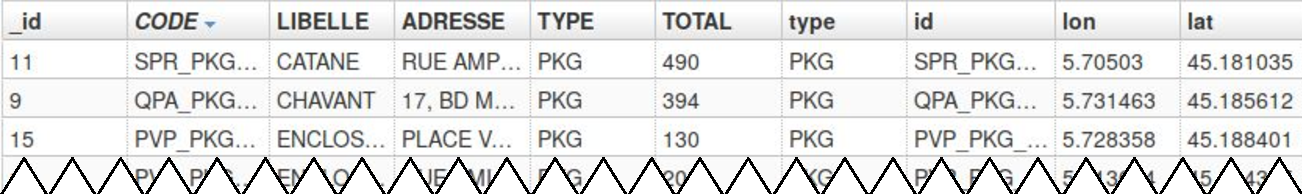
\includegraphics[scale=0.45]{images/sampleRawData.pdf}
	\caption{Parking data from Grenoble Open Data Portal}
	\label{fig:sampleRawData}
\end{figure}

\figref{sampleOntologyRawData} shows a possible vocabulary, that we refer to as a final mapping, for describing the parkings in \figref{sampleRawData}. The light blue and orange arrows are data and object properties respectively. As we can see, the final mapping reuses terms from several ontologies. The prefixes in the IRIs of ontology entities are shown in \reftab{prefixList}. Throughout this document, we use prefixes from this table. Also, below the IRIs of most ontology entities in \figref{sampleOntologyRawData}, the green labels refers to schema elements (i.e. column headers) in the parking data (\cf \figref{sampleOntologyRawData}) and above them is the ontology entity to which they have been mapped.

In our approach, formally described in \secref{approach}, the final mapping contains at least a class to type objects in the raw data and ontology entities that describe  objects' properties. For example, in \figref{sampleOntologyRawData}, we use \kword{mv:ParkingFacility} to type the objects in \figref{sampleRawData} and, the data property \kword{wgs84:long} and class \kword{mv:Capacity} are used to model their \kword{lon} and \kword{TOTAL} property respectively. Additionally, the latter ontology entities must be related to the latter classes used for typing directly or indirectly via other ontology entities. \kword{wgs84:long} is directly related as its domain include \kword{mv:ParkingFacility}. \kword{wgs84:long} can be used directly to specify the values as its domain include \kword{mv:ParkingFacility}. Nevertheless, for \kword{mv:Capacity}, the final mapping includes \kword{mv:capacity} to link to \kword{mv:ParkingFacility} and the data property \kword{mv:maximumValue} to specify the values.  



\begin{comment}
To express the values of the object's properties in the raw data, we use data properties or classes that are in the domain of a data property. For example, in \figref{sampleOntologyRawData}, \kword{lon} is modeled using the data property \kword{wgs84:long} that is used to specify the \kword{lon}'s values. Also, \kword{TOTAL} is modeled using the class \kword{mv:Capacity}. This class is the domain of the data property \kword{mv:maximumValue}.Therefore, the data property is used to specify the \kword{TOTAL}'s values. Moreover, \kword{wgs84:long} has been used as it is in the domain of \kword{mv:ParkingFacility}. Also, \kword{mv:capacity} is added to the \descriptionVocabulary as it relates \kword{mv:ParkingFacility} to \kword{mv:Capacity}.
\end{comment}

%Additionally, in our approach, the \descriptionVocabulary must be coherent. 

%More explicitly, entities in \descriptionVocabulary to represent the relation between the type and considered entities. 



\begin{figure}[h]
	\centering
	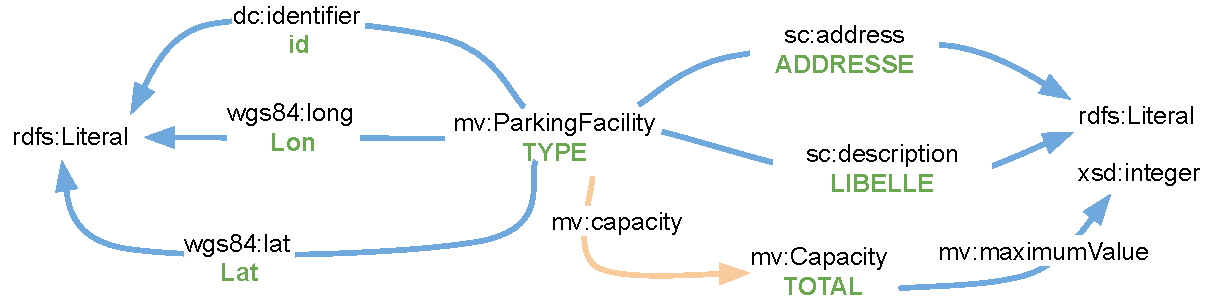
\includegraphics[scale=0.5]{images/sampleOntologyRawData.pdf}
	\caption{Vocabulary to describe parking data}
	\label{fig:sampleOntologyRawData}
\end{figure}
%The parking description reflects some important design decisions in our approach. First, as we can see, 

\begin{table}[]
	\centering
	\begin{tabular}{|l|l|l|}
		\hline
		\textbf{Prefix} & \textbf{Vocabulary Name} & \textbf{Namespace IRI}                       \\ \hline
		xsd             & XML Schema Definition    & http://www.w3.org/2001/XMLSchema\#           \\ \hline
		rdfs            & RDFS                     & http://www.w3.org/2000/01/rdf-schema\#       \\ \hline
		owl				& Web Ontology Language    & http://www.w3.org/2002/07/owl\#               \\ \hline
		sc              & Schema.org               & http://schema.org/                           \\ \hline
		mv              & MobiVoc                  & http://schema.mobivoc.org/                   \\ \hline
		
		wgs84           & WGS84                    & http://www.w3.org/2003/01/geo/wgs84\_pos\#   \\ \hline
		dc           & Dublin Core Metadata Terms                    & http://purl.org/dc/terms/   \\ \hline
		ign           & IGN administrative units                    & http://data.ign.fr/def/topo   \\ \hline
		
	\end{tabular}
	\caption{List of Vocabulary Prefixes}
	\label{tab:prefixList}
\end{table}



	
	
	       

\input{implementation.tex}


\section{Demonstration}\label{sec:demonstration}
%Our demonstration consist of using datasets from open data portals for some cities in France. \figref{expMappingParking} shows some of our experiments using these datasets. For each city, we performed two experiment. In \kword{NK}, no keywords are added by the user while in \kword{WK}, keywords are added. As we can see, even without keywords, there are fields that can be correctly mapped. Obviously, with keywords, initial mappings with better quality are generated. For all these datasets, we have their respective schema descriptions that we intend to use in our demonstration. 



%\begin{figure}
%	\centering
%	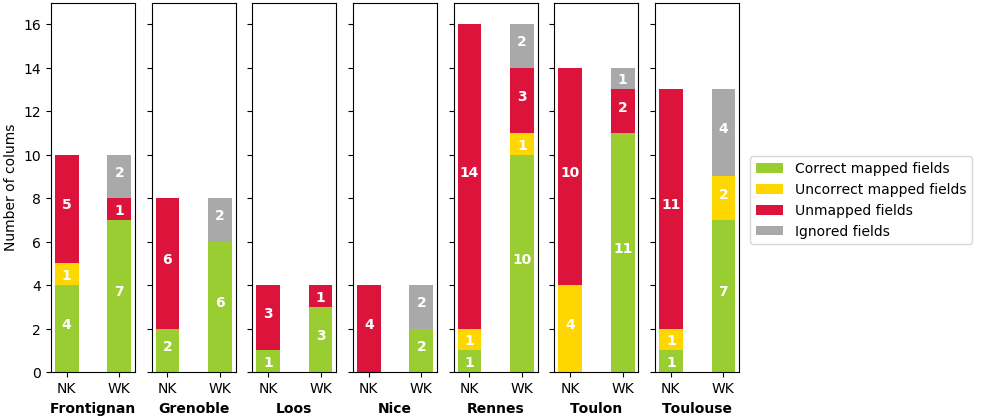
\includegraphics[scale=0.3]{./images/mappingPerParking1.png}
%	\caption{Mappings of the columns grouped per parking dataset. Where \emph{NK} represents the 
%		experiment without keywords and \emph{WK} represents the experiments with keywords.}
%	\label{fig:expMappingParking}
%\end{figure}

During this demonstration, we intend to RDFize Grenoble parking dataset partly shown in \figref{sampleRawData}. We perform two experiments: \kword{NK}and \kword{WK}. In \kword{NK}, we only specify the \kword{type description} with keywords. In \kword{WK}, we also specify keywords for interested columns. These keywords are shown in \tabref{overviewElementMappings}. Results are despicted in Table~\ref{tab:expGrenoble}. As we can see in \tabref{expGrenoble} and the video, adding keywords greatly improve the quality of mappings that are generated.

%\vspace{-0.5cm}

\section{Conclusion}
We have tested our approach on real datasets from open data portals and the results were promising. However, there are three main limitations. Firstly, the success of the approach depends much on the selection of keywords. It may not be easy for the user to define the keywords that will correspond to labels of ontologies entities. A extension of the approach that will suggest keywords according to these labels is currently being implemented. Secondly, as mentioned in \secref{approach}, our approach can consider raw data containing only one type of object described by several data properties. However in some cases, the object can be link in its description to other objets. Approaches dealing with entity resolution and entity linking could be used.  
Thirdly, as of now, there are no alignments between the ontologies in the ontology repository. The existence of these alignments can improve the quality of the generated mappings.



\begin{table}[]
    \centering
    \begin{tabular}{|c|c|c|c|c|c|c|}
        \hline
         &   LIBELLE & ADRESSE & TOTAL & id & lon & lat \\
        \hline
        NK & -- & schema:adress & --&  mobivoc:id & -- & -- \\
        \hline
        WK & schema:label & schema:adress & mv:Capacity & dc:id & geo:long & geo:lat \\
        \hline
    \end{tabular}
    \caption{Initial mappings without keywords (\texttt{NK}) and with keywords (\texttt{WK})}
    \label{tab:expGrenoble}
\end{table}
\vspace{-0.5cm}
\input{conclusion.tex}




\bibliographystyle{unsrt}
\bibliography{references}
\end{document}
